\documentclass[12pt]{article}
\usepackage{listings}
\usepackage{hyperref}
\usepackage{graphicx}
\title{EARIN project Midterm report}
\author{Krzysztof Rudnicki \\ Jakub Kliszko}
\begin{document}
\maketitle
\section{Progress}
We have implemented reading data from csv files, preprocessing them with optional showing of some of the information about the data and used model/learner for implementing neighbour searches \\ 
Program is very flexible and allows for a lot of modification from command line arguments \\
Full list here:
\begin{lstlisting}[language=bash]
options:
-h, --help            show this help message and exit
--data_limit DATA_LIMIT, -dl DATA_LIMIT
                      Specify data limit, Recommended at least 500k,
                      set to -1 for no limit
--seed SEED, -s SEED  Specify seed
--debug DEBUG, -d DEBUG
                      Use debug (more information) prints
--database DATABASE, -db DATABASE
                      Specify database path
--metric {cosine,mahalanobis,euclidean}
-m {cosine,mahalanobis,euclidean}
                      Specify metric for NearestNeighbor learner
--algorithm {auto,ball_tree,kd_tree,brute}
-a {auto,ball_tree,kd_tree,brute}
                      Specify algorithm for Nearest Neighbor learner
--anime ANIME, -an ANIME
                      Specify anime to choose
--neighbors NEIGHBORS, -n NEIGHBORS
                      Specify number of nearest neighbors
--user_threshold USER_THRESHOLD, -ut USER_THRESHOLD
                      Specify minimal number of votes
                    required for user to be included in
                    the data, set to -1 for no threshold
--anime_threshold ANIME_THRESHOLD, -at ANIME_THRESHOLD
                      Specify minimal number of votes
                      required for anime to be included
                      in the data, set to -1 for no threshold
\end{lstlisting}
\section{Results}
Currently recommendations are displayed in a following way: 
\begin{lstlisting}[language=bash]
Recommendations for Kill la Kill:

1: Shingeki no Kyojin, with distance of 0.11106648055176693:
2: Steins;Gate, with distance of 0.12104265014640536:
3: Toradora!, with distance of 0.12112848901274798:
4: Sword Art Online, with distance of 0.13046005032340824:
5: No Game No Life, with distance of 0.1306815843129835:
6: One Punch Man, with distance of 0.14848484728234945:
7: Angel Beats!, with distance of 0.15175709939974935:
8: Hataraku Maou-sama!, with distance of 0.15244674042590045:
9: Psycho-Pass, with distance of 0.15288022814590008:
  \end{lstlisting}
  Where we are given name of the anime for which we create recommendation and list of animes recommended with distance to original anime (lower is better)
  \subsection{Data size and execution time}
  \begin{figure}
    \caption{Chart showing how size of data taken impacts execution time }
    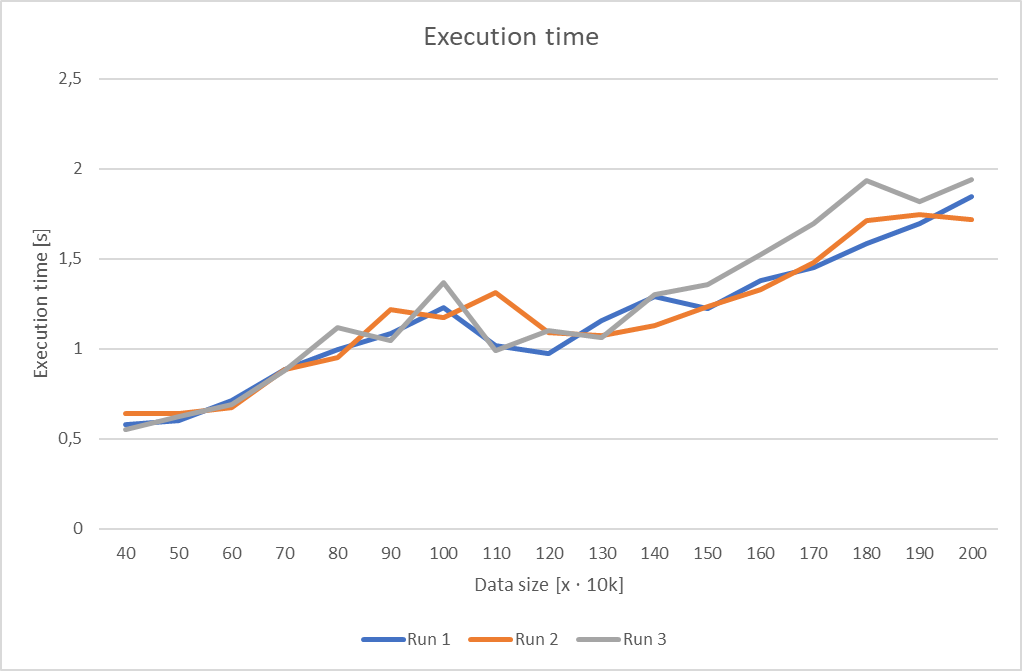
\includegraphics[width=\textwidth]{execution_time.png}
  \end{figure}
This data was taken using default parameters execpt for increasing data size, each of three runs uses different seed


\paragraph{Seed} We added seed in predict function for choosing random anime, using the same seed always returns same recommendations and choosing random anime is the only random part of our code \\ 
User can specify their own seed by using -s or --seed flag by entering in command line:
\begin{lstlisting}
python -s 42
\end{lstlisting}
\section{Challenges}
\subsection{Failed attempts}
Biggest challenge was realizing how overcomplicated and unnecessary difficult to implement is the first code we based on: \href{https://www.kaggle.com/code/chaitanya99/recommendation-system-cf-anime}{Kaggle code with tensorflow} \\ 
This solutions runs for almost 10 minutes on kaggle and implementing it to run on our local devices was a real chore that took us a good day and a half to implement \\
This implementation is based around very powerful Tensor Processing Unit from google and while it is possible to change it to run on local graphics card it requires downloading both cuda and cudnn to a downgraded version supported by tensorflow (11.8) and downgrading graphics card drivers \\ 
Running it with CPU results in the model training for over 3 hours 
\subsection{Corrections}
Suprisingly even though we based our preliminary report around different example code we managed to not make any corrections to preliminary report \\ 
All of functionality that we want to implement is available in sklearn and scipy 
\subsection{Results and findings}
We can see that the rating is skewed towards higher values, users tend to give ratings of 7, 8 or 9 which inflates average rating to be well above 5
\begin{figure}
  \caption{User rating count}
  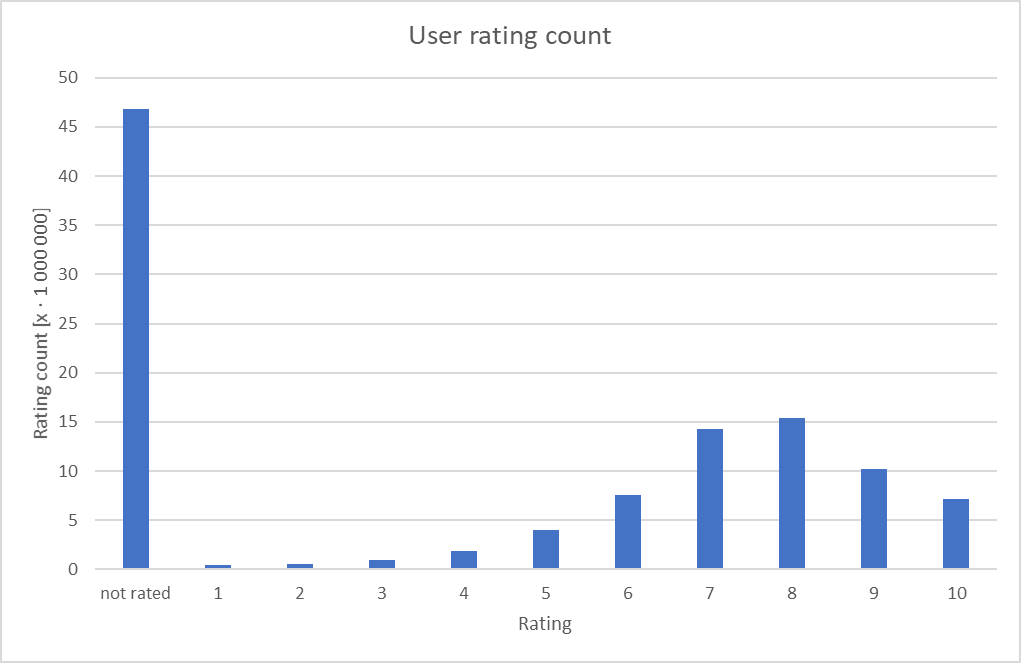
\includegraphics[width=\textwidth]{user_rating.png}
\end{figure}
\section{Finishing project}
\subsection{Embedding more data in user and anime}
Currently we are only embedding pure rating values of users, we do not take into consideration, popularity, "controversy", studio which created the anime, length of anime (number of episodes and length of episodes), and when it was aired \\ 
\subsection{Evaluating our model accuracy}
We need to introduce some way to evaluate accuracy of our model, we will try to introduce at least some of the measures mentioned in preliminary report: precision, recall, F1 score and MAP
\subsection{More results representation}
We still need to introduce more representation for our model results. Mainly how well it predicts similarity based on different parameter values (different modes, arguments and so on) \\ 
We already can modify those values easily from the code itself and as argument, we just need to run those values and collect results


\end{document}